\documentclass[a4paper]{oblivoir}
% define the title
\author{Moon Il-chul \\ \href{mailto:icmoon@kaist.ac.kr}{icmoon@kaist.ac.kr} 
   \and Jang Jae-kwan \\ \href{mailto:jgfd123@gmail.com}{jgfd123@gmail.com} }
\setcounter{chapter}{1}
\title{Chapter 1. 동기 및 기본지식}
\usepackage{indentfirst}
\usepackage{graphicx}
\graphicspath{ {Figure/} }
\usepackage{hyperref}
\usepackage{amsmath}
\usepackage{amssymb}
\usepackage{amsfonts}
\usepackage{dsfont}
\usepackage[]{algorithm2e}
\usepackage{chngcntr}
\counterwithin{figure}{chapter}
\setcounter{tocdepth}{2}
\setcounter{secnumdepth}{3}
\hypersetup{pdfborder={0 0 0}}
\renewcommand{\thefigure}{\thechapter-\arabic{figure}}
\renewcommand{\theequation}{\thechapter.\arabic{equation}}
\newlength\myindent
\setlength\myindent{5em}

\begin{document}
% generates the title
\maketitle
%\renewcommand{\contentsname}{목차}
\tableofcontents
%\listoftables
%\listoffigures

%슬라이드 3
\section{동기}

%슬라이드 4,5
\subsection{기계학습 예시}
요즘 여러 사람들이 기계학습과 관련되어 다양한 키워드를 말하고 있는데 데이터마이닝(Data-mining), 기계학습(Machine Learning), 인공지능(Artificial Intelligence) 등이 있다. 즉, 여러 다양한 분야에서 연구를 진행하고 있어서 다양한 키워드들이 혼재하고 있다. 앞으로 이 책에서는 "기계학습(Machine Learning)"으로 언급을 하겠지만 다른 키워드로 얘기를 하여도 무방하다. 현재 기계학습 분야가 많이 활성화 되고 있는 이유는 상당히 많은 데이터들이 축적이 되었고 또 공개된 데이터들도 많아졌기 때문이다. 또한 이를 처리할 수 있는 능력이 생겨나고 있다는 이유가 있다.\\
%슬라이드 6
\begin{figure}[ht]\centering
\parbox[t]{3.5cm}{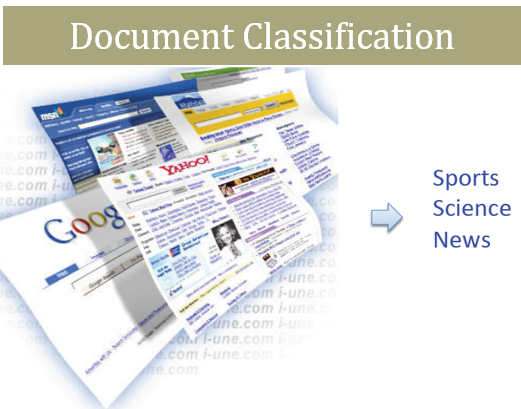
\includegraphics[scale=0.45]{Document}\caption{문서 분류\label{Fig:1-1}}}\hspace{2cm}
\parbox[t]{5cm}{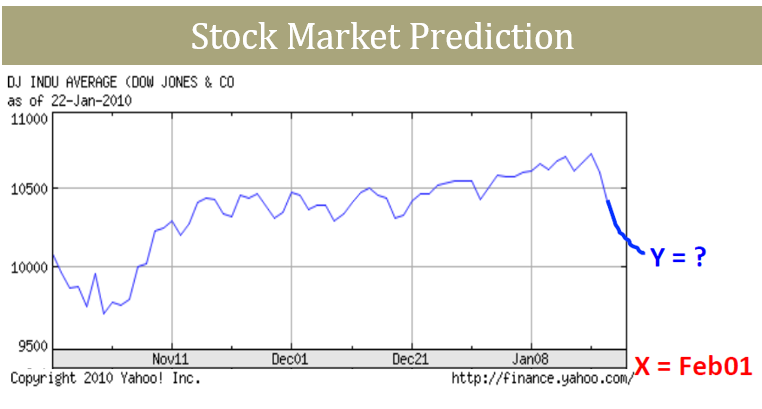
\includegraphics[scale=0.45]{Stock}\caption{주가 예측\label{Fig:1-2}}}
\parbox[t]{3.5cm}{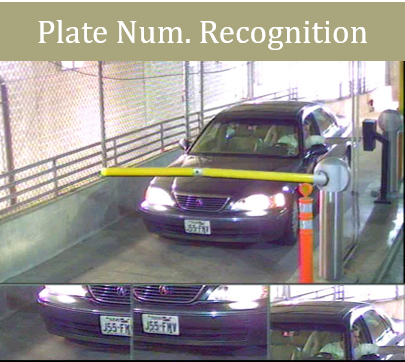
\includegraphics[scale=0.45]{Car}\caption{번호판 인식\label{Fig:1-3}}}\hspace{0.2cm}
\parbox[t]{5.5cm}{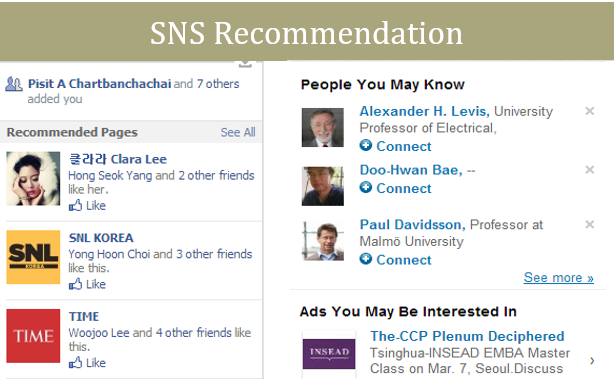
\includegraphics[scale=0.45]{SNS}\caption{SNS 추천\label{Fig:1-4}}}
\parbox[t]{2.5cm}{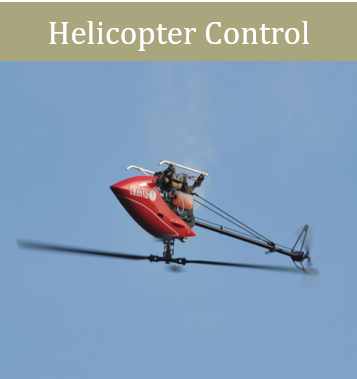
\includegraphics[scale=0.45]{Helicopter}\caption{헬리콥터 조정\label{Fig:1-5}}}
\end{figure}\\
\indent 기계학습의 적용 예시들은 매우 다양하다. 이메일을 받을 때 스팸메일을 안 받게 하는 작업, 주식시장에서 주가를 예측하는 작업, 자동차 번호판 자동 인식방법, SNS 상에서 팔로우 대상을 추천하는 시스템, 헬리콥터(로봇)를 공중에서 자동으로 조정하는 시스템 등에서 기계학습이 적용이 되고 있다. \\
%슬라이드 7
\begin{figure}[ht]\centering
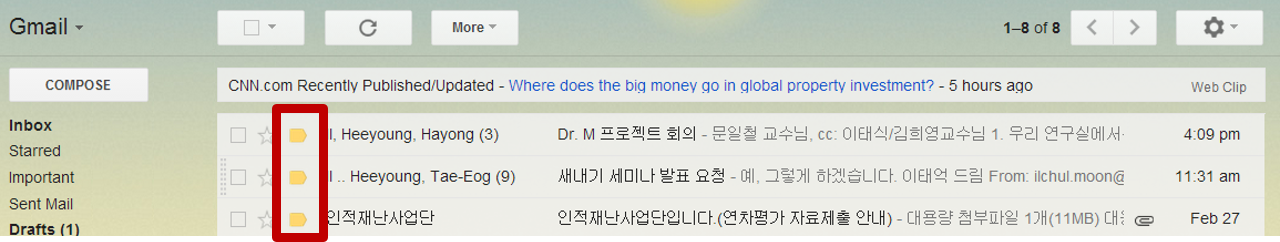
\includegraphics[scale=0.45]{Spamfiltering}\label{Fig:1-6}
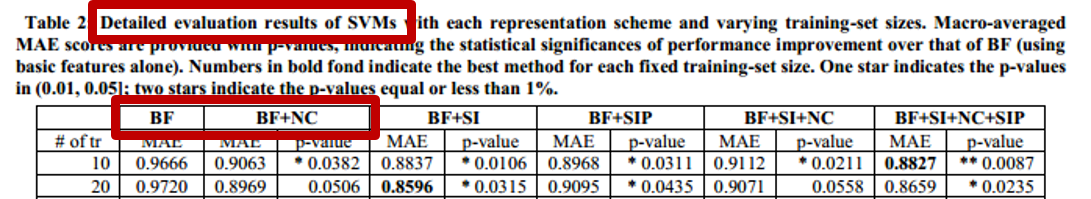
\includegraphics[scale=0.45]{Spamfiltering2}\label{Fig:1-7}
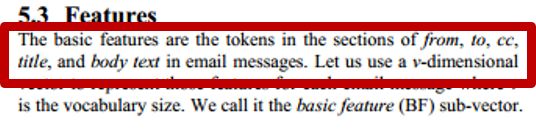
\includegraphics[scale=0.45]{Spamfiltering3}\label{Fig:1-8}
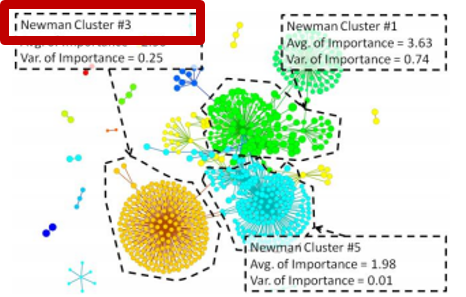
\includegraphics[scale=0.45]{Spamfiltering4}\label{Fig:1-9}
\caption{이메일 스팸 차단 및 중요성 표시}
\end{figure}\\
\indent 예전에는 이메일에서 스팸 필터링만 하였는데, 최근 특정 사이트에서는 이메일에 중요도를 판별하여 표시하는 시스템이 갖춰져 있다. 이와 같은 시스템은 이메일 안에 있는 여러 가지 텍스트 정보를 이용하기도 하고, 메일 간의 소셜 네트워크를 활용하기도 한다. 또한 앞의 두 데이터를 합치면서 몇 가지 기계학습 기법을 적용하여 만들어낸 결과물이다.\\
%슬라이드 8
\begin{figure}[ht]\centering
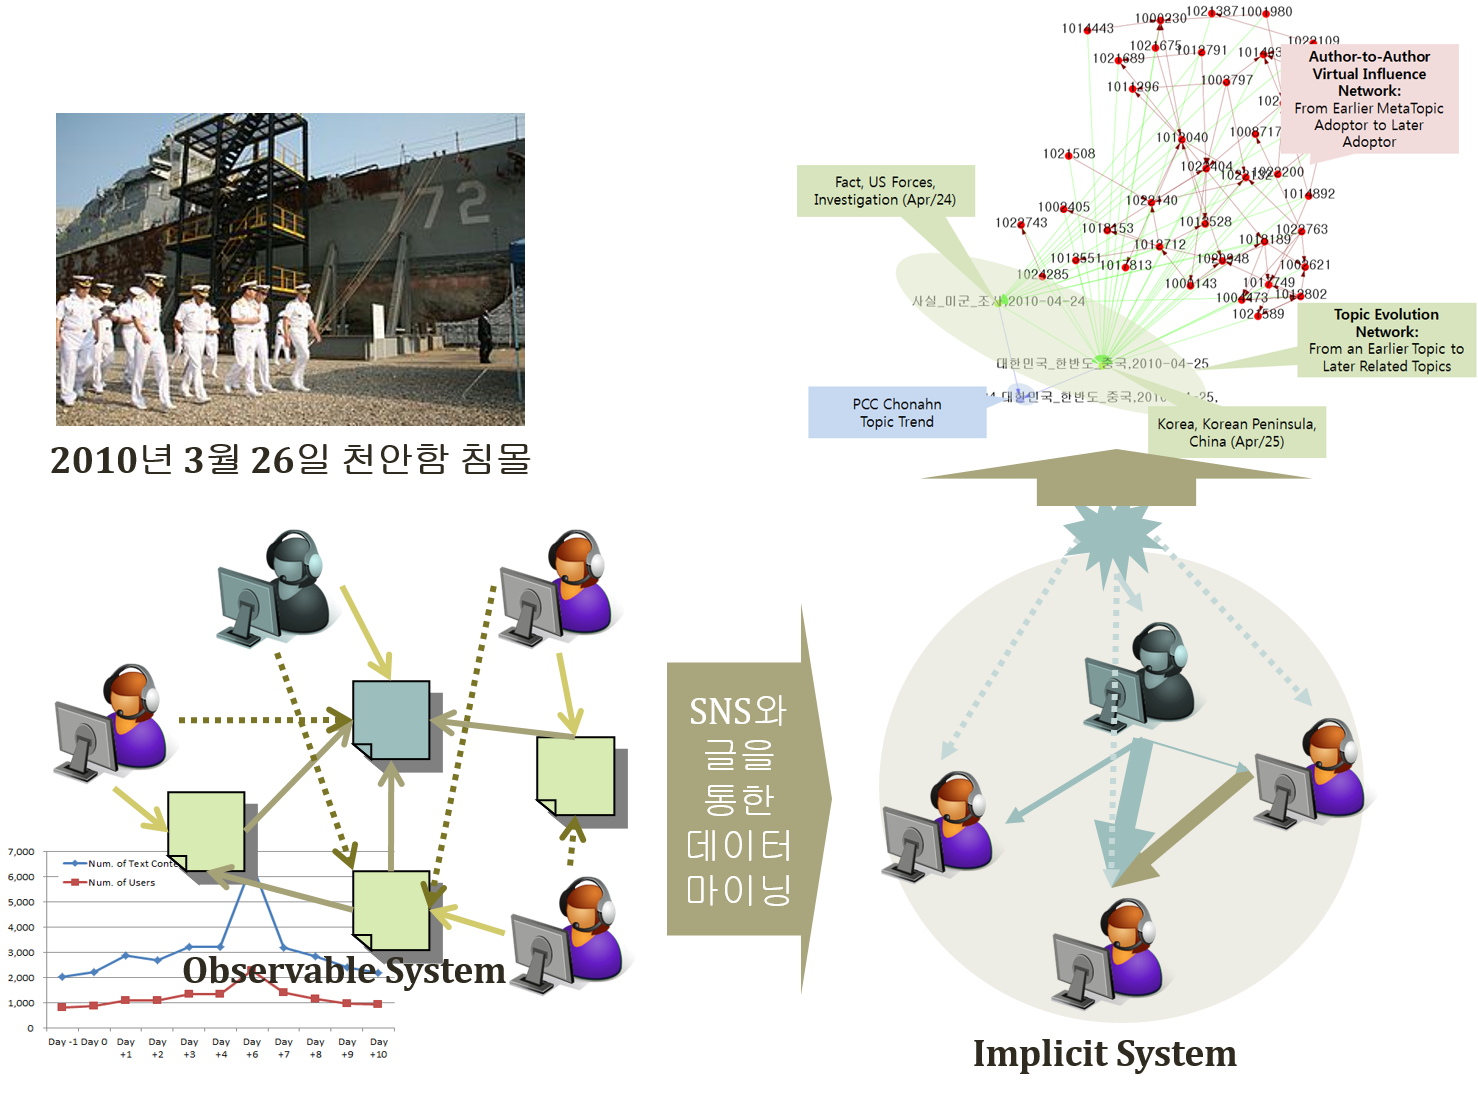
\includegraphics[scale=0.5]{Opinionmining}\caption{오피니언 마이닝}\label{Fig:1-10}
\end{figure}\\
\indent 2010년 천안함 침몰 당시 다양한 소셜 네트워크 정보들을 모아 어떤 시기에 어떤 글들이 많았는지 정보를 뽑아 낼 수 있었다. 이 정보를 토대로 기계학습을 이용하면 어떤 주제들이 돌아다니고 있는지, 그리고 이 주제들이 다른 사람들에게 어떻게 전파되는지를 파악할 수 있다. 이를 오피니언 마이닝이라고 하며 이를 통해 다수의 의견을 찾아낼 수 있고,  특정 사건에 대한 사람들의 인식을 모아볼 수 있다. 즉, 많은 데이터 속에서 중요한 의견을 모을 수 있고, 한 집단에서 앞으로의 대립 관계를 예측해볼 수 있다. 이를 통해 집단의 통합을 유지하기 위한 전략을 짤 수 있다.\\
%슬라이드 9
\begin{figure}[ht]\centering
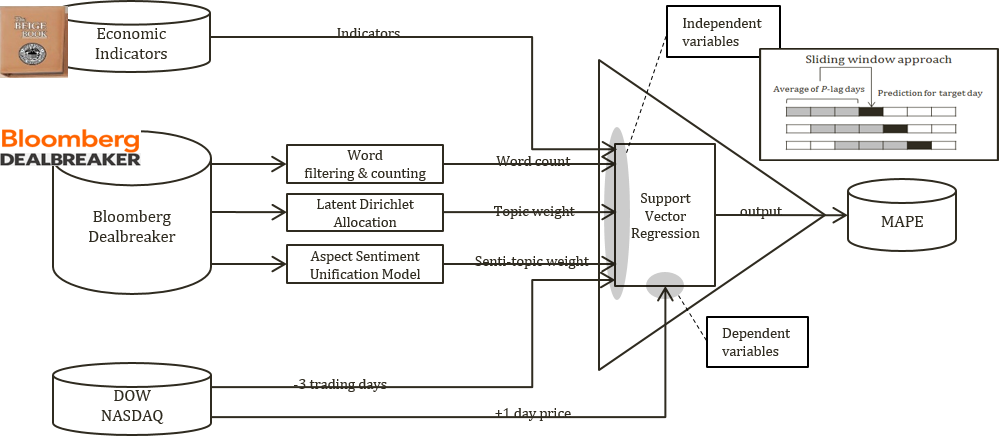
\includegraphics[scale=0.5]{Stockmarket}\caption{주식 시장}\label{Fig:1-11}
\end{figure}\\
\indent 또한 다양한 경제 지표와 경제 뉴스를 활용하여 하나의 기계학습 테크닉으로 묶고, 이를 토대로 내일의 주가 지수 등을 예측해볼 수 있다.
\begin{figure}[ht]\centering
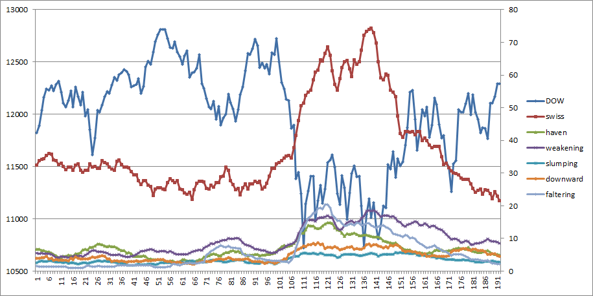
\includegraphics[scale=0.5]{Stockmarket2}\label{Fig:1-12}
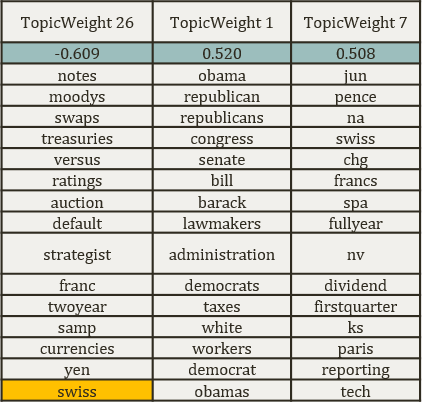
\includegraphics[scale=0.5]{Stockmarket3}\label{Fig:1-13}
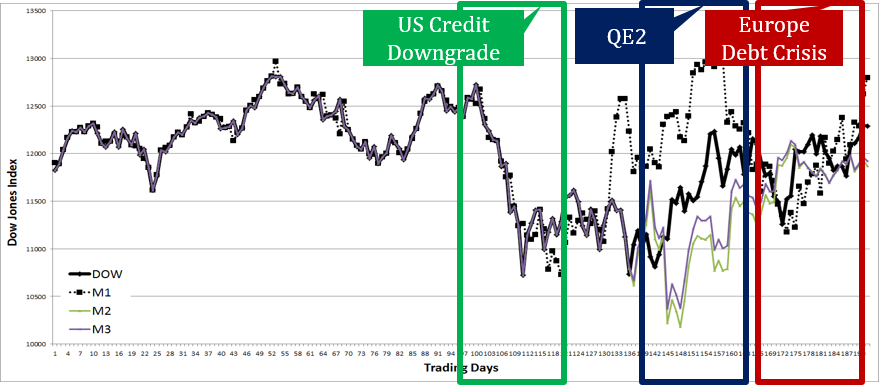
\includegraphics[scale=0.5]{Stockmarket4}\label{Fig:1-14}
\caption{“swiss” 와 DJIA 간의 강한 음의 상관관계}
\end{figure}
필자는 이와 관련된 연구를 진행하였는데, DJIA(다우존스 산업평균지수)와 "swiss"라는 단어는 음의 상관관계를 가진다는 결과를 얻었다. 좀 더 살펴보면 기계학습 결과에서  "swiss","yen","franc" 등이 함께 있는 토픽이 증가할 때 DJIA는 감소하게 되었다. 그 이유는 DJIA가 떨어지면 주식에 투자했던 사람들이 좀 더 안전한 자산으로 옮기려 하기 때문에 일본의 엔화나 스위스의 프랑화를 찾게 되어 강한 음의 상관관계가 생성이 되는 것이다.
%슬라이드 10
\subsection{기계학습 종류}
기계학습의 종류에는 크게 지도학습과 자율학습, 강화학습이 있다. 지도학습은 몇몇 경우에 대해 답을 알고 있는 상황에서 답을 예측하고 맞추는 분야이다. 자율학습은 답을 모르는 상황에서 집단을 요약하고 대표를 찾고 군집을 찾아내는 분야이다. 강화학습은 목적은 알지만 어떻게 달성해야할지 모를 때 쓰이는 분야이다. 이 외에도 다양한 학습 방법이 존재한다. 앞으로 이 책에서는 지도학습과 자율학습에 대해 자세히 알아보고자 한다. 강화학습의 경우에는 성격이 다르기도 하고 로봇과 연관되는 부분이 많아 이 책에서는 다루지 않을 것이다.\\
\begin{figure}[ht]\centering
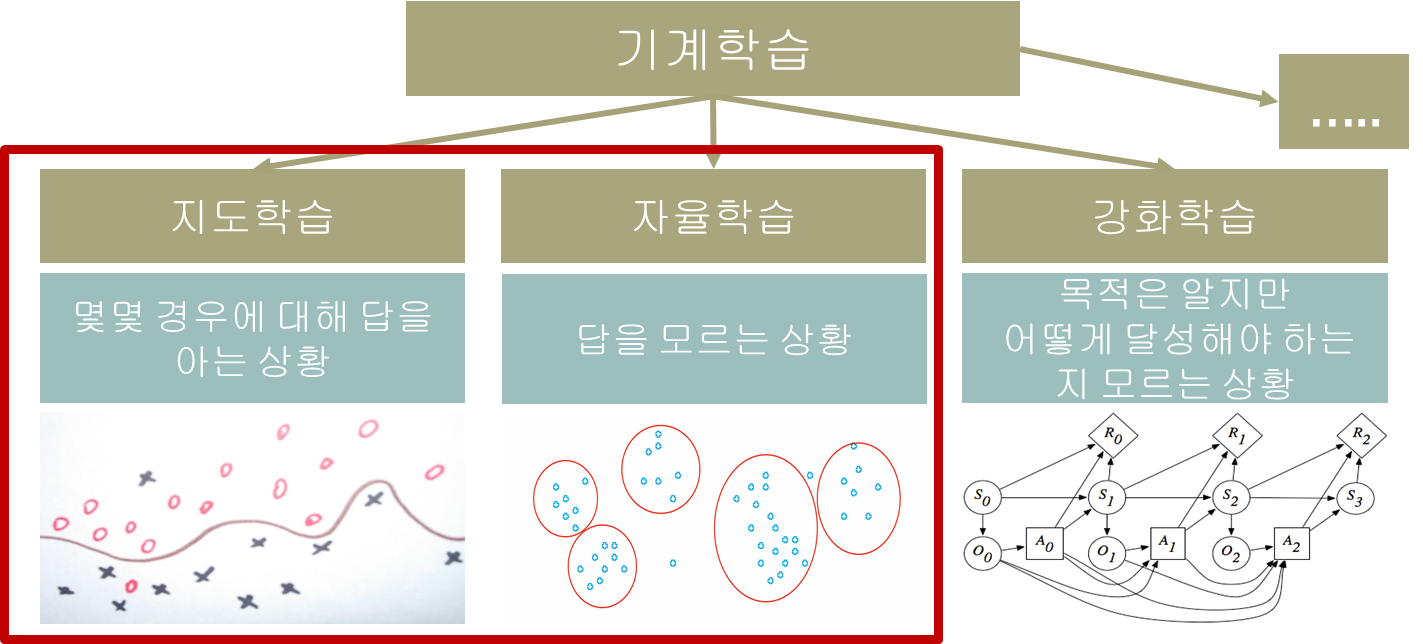
\includegraphics[scale=0.5]{Machinelearning_Type}\caption{기계학습의 종류}\label{Fig:1-15}
\end{figure}\\
%슬라이드 11
\indent 지도학습은 사람이나 데이터 등을 통한 감독이 가미된 기계학습이다. 이 학습의 경우에는 찾고자 하는 대상(값)을 있고, 이에 해당하는 예시를 제공 가능한 경우에 해당한다. 예를 들어 스팸 필터링에서는 메일 중 차단하고자 하는 대상이 있고, 자동등급판정 혹은 자동범주화에서는 분류하고자 하는 대상이 있다. 아마존에서는 제품 분류를 할 때, 마지막으로 사람의 손을 거쳐 분류하기전에 제품의 정보를 받아  미리 자동으로 분류를 하는 것이 이에 해당한다. 지도학습의 방법론에는 크게 Classfication(분류)와 Regression(회귀분석)로 나눌 수 있다. 분류는 관측으로부터 이산형 종속 값을 추정하는 것이고 회귀분석은 연속형 종속 값을 추정하는 것이다. 분류의 예시로는 어떤 대상이 맞는지 틀리는지 구분하는 경우도 있고, 등급을 매길 때 몇몇 경우에 대한 값을 입력하여 이 정보가 감독하에 입력하지 않은 값에 대한 등급을 매기는 예시도 있다. 또한 특정 글이 긍정적인지 부정적인지 판단을 내리는 알고리즘도 있을 수 있다. 회귀분석의 예시로는 주식 시장에서 다음날의 주가를 예측하는 알고리즘이 있다.\\

%슬라이드 12
\indent 자율학습은 참값을 모르는 상황에서 별다른 통제 없이 인공지능이 오로지 주어진 데이터를 활용해 군집을 찾고 패턴을 찾는 기계학습이다. 자율학습의 경우에는 군집을 찾는 때 쓰일 수 있고, 잠재적 요인이나 그래프 구조를 찾고 싶을 때 사용이 된다. 예를 들어 수 많은 기사들을 주제 10개로 요약하는 것은 군집을 찾는 과정으로 볼 수 있고, 여러 사람의 얼굴을 모아 군집을 만들었을 때 잠재적으로 숨어 있는 잠상을 찾는 알고리즘도 예시 중 하나이다. 또 다른 예시로 다 완성되지 않은 상품 평가 점수 표에서 남은 칸은 채우는 자율학습도 있고, 궤적 데이터에서 노이즈를 필터링 하는 자율학습도 있다. 자율학습의 방법론에는 클러스터링과 필터링이 있다. 클러스터링은 세트를 예측하고 각 사례들을 세트에 넣는 방법이고, 필터링은 신호와 노이즈가 섞여있는 것으로부터 근본적이고 기본적인 신호를 예측하는 방법이다.\\\\

\section{기본 지식}
%슬라이드 13
\subsection{간단한 확률 예시}

%슬라이드 14,15
기계학습에서는 확률이 중요하기 때문에 확률에 관해 간단히 알아보는 과정을 거치려고 한다. 이를 위해 간단한 확률 문제를 생각해보려고 한다. 압정을 던져서 나오는 결과에 따라 돈을 따는 도박 사이트가 있다고 생각을 해보자. 이 사이트에서는 압정의 못 부분이 위로 갈지 아래로 갈지 정확히 예측해 맞춘다면 베팅한 금액을 두배로 벌 수 있다고 한다. 그리고 한 억만장자가 이 도박에 참가하고자 하여 당신에게 많은 돈을 주며 과학적이고 공학적인 분석을 요구했다고 생각해보자. 이 억만장자는 도박에 쓰이는 못을 구해왔고, 당신에게 못이 위를 향할 확률이 얼마나 되는 지를 물어봤다면 당신의 대답은 무엇인가?\\
\begin{figure}[ht]\centering
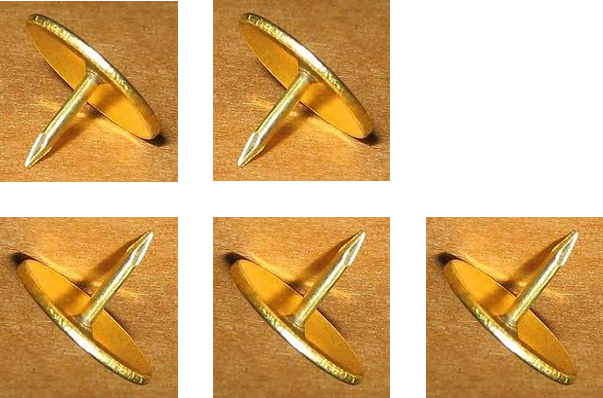
\includegraphics[scale=0.5]{Thumb}\caption{압정을 5번 던진 결과}\label{Fig:1-16}
\end{figure}\\
\indent 보통의 경우 대답은 몇 번 던져보자는 대답이 나올 것이다. 그래서 억만장자는 이 압정을 5번 던져보았다. 그 중 3번이 못이 위를 향했다고 한다. 하지만 이 결과를 보고 바로 못이 위를 향할 확률이 3/5라고 말을 하기는 힘들 것이다. 그 이유에 대해서 물어볼 경우 명확히 답할 수 없기 때문이다. 이제는 이 이유에 대해 명확히 답할 수 있는 방법에 대해 알아보도록 하겠다.\\

%슬라이드 16
\indent 이를 위해서는 이항분포에 대해 알아야한다. 이항분포는 결과가 Yes or No로 2가지로 정해져 있는 상황에서 n번의 독립적인 실험을 했을 때 성공한 횟수에 대한 이산확률분포이다. 그리고 각각의 실험에서 성공의 확률은 $\theta$이다. 또한 이는 베르누이 실험이라고 불린다. 그리고 압정을 던졌을 때 각각의 실험은 I.I.D를 만족함을 가정한다. IID는 Independent Identically Distributed의 약자로써 각 사건은 독립적이고 동일한 분포를 나타냄을 의미한다.\\\\
\indent 압정의 못이 위를 바라보는 사건을 $H$, 아래를 바라보는 사건을 $T$로 정의하고, $H$가 나올 확률을 $P(H)=\theta$라고 가정하면 $T$가 나올 확률은 $P(T)=1-\theta$가 된다. 그 이유는 한번의 실험에 대해서 나올 수 있는 모든 경우의 확률을 더했을 때는 1이 되어야 하기 때문이다. 앞선 가정을 만족한 상황에서 모든 실험은 독립적이고 동일한 확률을 가지므로 압정을 5번 던진 경우 결과가 HHTHT가 나올 확률은 다음과 같다.\\
\begin{equation}
P(HHTHT)=\theta\theta(1-\theta)\theta(1-\theta)=\theta^3(1-\theta)^2
\label{eq:1-1}
\end{equation}
\indent여기서 5번 던진 결과(Data)를 $D$로 두고, 던진 횟수는 $n=5$, 못이 위를 향한 횟수는 $k=a_H=3$, 못이 위를 향할 확률은 $p=\theta$로 정의를 해보자. 그렇다면 압정의 못이 위를 향할 확률이 $\theta$로 주어졌을 때, $D$ 결과가 나올 확률은 다음과 같다.\\
\begin{equation}
P(D| \theta)=\theta^{a_H}(1-\theta)^{a_T}
\label{eq:1-2}
\end{equation}
\indent 이 값은 H가 나올 확률에 H가 나온 횟수만큼 제곱하고, T가 나올 확률에 T가 나온 횟수만큼 제곱한 값을 곱한 결과이다. 이 식을 좀 더 일반화 시키면 다음과 같다.\\
\begin{equation}
f(k;n,p)=P(K=k)={\binom{n}{k}}p^k(1-p)^{n-k}
\label{eq:1-3}
\end{equation}
\indent 여기서 n은 실험의 횟수, p는 성공할 확률로써 주어진 변수이다. 그리고 확률은 성공한 횟수인 k의 값에 따라 계산된다. 이때 k번 성공할 확률은 성공할 확률에 성공한 횟수만큼 제곱하고, 실패할 확률에 실패한 횟수만큼 제곱한 뒤, n번 중 k번이 언제 성공할 지 조합을 계산하는 $nCk$를 곱해주면 된다.\\
\begin{equation}
nCk={\binom{n}{k}}=\frac{n!}{k!(n-k)!}
\label{eq:1-4}
\end{equation}\\

\subsection{MLE}
%슬라이드 17
앞서 압정을 던져 위를 향할 확률이 $\theta$ 로 주어졌을 때, $D$ 라는 데이터가 관측될 확률은 수식 \eqref{eq:1-1}과 같다고 하였다.\\
\begin{figure}[ht]\centering
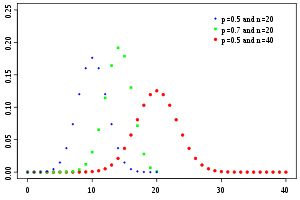
\includegraphics[scale=1]{bino}\caption{이항분포 예시}\label{Fig:1-17}
\end{figure}\\
\indent 여기서 우리의 가정은 압정의 도박 결과는 $\theta$라는 이산확률 분포를 따른다는 것이였다. 그렇다면 어떻게 하면 우리의 가정이 강해질까? 어떻게 하면 가정이 강해져서 우리의 주장이 참이라고 말할 수 있을까? 먼저 이항분포보다 더 나은 분포를 찾을 수도 있다. 하지만 여기에 대해서는 좀 더 합리적인 생각이 필요하다. 또 다른 방법으로는 이항분포를 따르는 것은 인정하고, 가장 나은 $\theta$ 후보자를 찾아내는 것이다. 즉, 어떤 $\theta$를 선택을 했을 때 주어진 데이터를 가장 잘 설명할 수 있을 지를 찾는 것이다. 여기서 우리가 먼저 찾아볼 후보자는 $\theta$에 대한 최대우도추정(MLE)이다. MLE란 Maximum Likelihood Estimation이다. 이 방법은 관측된 데이터의 확률을 최대화하는 $\theta$를 찾는 것이다. 이를 수식으로 나타내면 다음과 같다.
\begin{equation}
\hat{\theta}={argmax}_{\theta}P(D| \theta)
\label{eq:1-5}
\end{equation}
\indent 이 수식을 좀 더 설명하자면, $P(D| \theta)$를 최대화 하는 $\theta$를 찾아내고 이를 $\hat{\theta}$라고 부르겠다는 의미이다. 여기서 $argmax$는 이 책에서 많이 쓰일 예정이므로 앞의 수식을 잘 이해하는 것이 좋다. 중요하기 때문에 좀 더 쉽게 풀어서 설명해보면, $\theta$가 주어졌을 때 데이터 $D$를 관측할 확률을 알 수 있고($P(D| \theta)$) 이를 최대화 하는 $\theta$를 역으로 찾아내고, 이를 $\hat{\theta}$로 부르겠다는 의미이다.

%슬라이드 18
이제 압정 문제에 MLE를 적용하여보겠다. 우선 $\hat{\theta}$를 정의하면 다음과 같다.
\begin{equation}
\hat{\theta}={argmax}_{\theta}P(D| \theta)={argmax}_{\theta}\theta^{a_H}(1-\theta)^{a_T}
\label{eq:1-6}
\end{equation}
\begin{figure}[ht]\centering
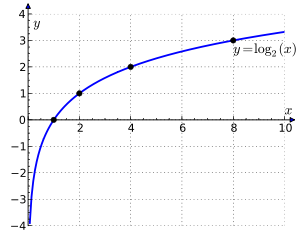
\includegraphics[scale=1]{Log_Function}\caption{로그함수 예시}\label{Fig:1-18}
\end{figure}
\indent 하지만 이 수식은 자승을 처리하기가 쉽지 않다. 그리서 우리는 약간의 트릭을 쓸 것이다. 통계학이나 기계학습에서 종종 쓰는 기법인데 log 함수를 이용하는 것이다. 로그함수는 다음과 같이 단조롭게 증가하기 때문에 $P(D| \theta)$가 최대가 되는 지점과 $\ln P(D| \theta)$가 최대가 되는 지점이 같다. 이를 이용하여 앞선 수식 \eqref{eq:1-6}을 발전시켜보면 다음과 같다.
\begin{equation}
\begin{split}
\hat{\theta}&={argmax}_{\theta}\ln P(D| \theta)\\
&={argmax}_{\theta}\ln\theta^{a_H}(1-\theta)^{a_T}\\
&={argmax}_{\theta}\{a_H\ln\theta+{a_T}\ln(1-\theta)\}
\end{split}
\label{eq:1-7}
\end{equation}
\indent 한편 이 수식은 극대화(최댓값) 문제로 볼 수 있다. 따라서 도함수를 이용하여 극점을 찾는 방법을 사용하면 된다. 그래서 $\theta$에 대해 미분을 하게되면 다음과 같은 결과가 나온다.
\begin{align}
\frac{d}{d\theta}(a_H&\ln\theta+a_T\ln(1-\theta))=0 \\
&\frac{a_H}{\theta}-\frac{a_T}{(1-\theta}=0 \\
&\theta=\frac{a_H}{a_T+a_H}
\end{align}
\indent 즉, $\theta$가 $\frac{a_H}{a_T+a_H}$을 만족할 때, MLE 관점에서 가장 나은 후보자가 된다. 따라서 $\hat{\theta}$는 다음과 같다.
\begin{equation}
\hat{\theta}=\frac{a_H}{a_H+a_T}
\label{eq:1-11}
\end{equation}\\

% 슬라이드 19
\indent 앞의 내용을 통해 우리는 억만장자에게 합리적인 이유를 들며 설명을 할 수 있다. 압정을 던져 나온 결과와 MLE 관점에서 보았을때, 확률분포가 이항분포라는 가정 하에서 우리는 $\theta$는 3/5=0.6이라고 말할 수 있다. 따라서 Head에 거는 것이 이길 확률이 높다고 말할 수 있다. 그래서 이와 같이 억만장자에게 설명을 했더니 이번에는 억만장자가 50번을 던져 보았다고 한다. 그리고 그 결과 30번 head가 나오고 20번 tail이 나왔다고 한다. 그리고 그렇다면 이 결과로 달라진 것이 없냐는 질문을 던졌다. 이때 당신은 어떻게 대답할 것인가?\\

% 슬라이드 20
\indent 당신은 ``더 많은 시도는 우리의 추정에 대한 에러를 줄일 수 있다.'' 라고 대답할 수 있다. 지금 수식 \eqref{eq:1-11}로 나타낸 $\hat{\theta}$은 추정한 것이고, 압정 던지기에 대한 실제 매개변수 $\theta^*$에 대해서 에러가 존재할 수 밖에 없다. 우리는 Hoeffding의 부등식을 이용해 확률에 대한 간단한 상한(upper bound)을 구할 수 있다. 다음 수식이 그 결과이다. 여기서 $N$은 던진 총 횟수이다.
\begin{align}
&N=a_H+a_T\\
&P(|\hat{\theta}-\theta^*|\geq\varepsilon)\leq2e^{-2N\varepsilon^2}
\end{align}
\indent 이 수식을 조금 살펴보면 $\varepsilon$이 커지게 되면 우변의 값은 작아지게 된다. 이 말은 Error Bound가 커지게 되면 좌변의 확률은 작아진다는 의미이다. 또한 $N$ 값이 커지게 되면 우변의 값은 작아지게 되고 좌변의 확률은 작아지게 된다. 이 말은 추정된 $\hat{theta}$와 실제 $\theta$가 차이가 작다는 의미가 된다. 만약 억만장자가 당신에게 추정 값과 실제 값의 차이인 $\varepsilon$가 0.1보다 클 확률이 0.01\%가 되기 위한 $N$ 값을 계산 할 줄 아냐고 물어본다면 물론 계산이 가능하다. 그리고 이 과정은 PAC learning 이라고 할 수 있다. 

% 슬라이드 21
\indent 기계학습 커뮤니티에서 Probably Approximately Correct(PAC) learning 이론은 학습자(learner)는 샘플 데이터를 받고, 특정 클래스의 사용 가능한 함수들로부터 일반화 함수와 가정을 고른다. 이런 선택된 함수는 높은 확률로 낮은 일반화 오류를 가지고 있다. 기계학습의 정의는 많은 관점에서 존재한다. Tom Mitchell은 다음과 같이 기계학습을 정의 하였다. ``컴퓨터 프로그램이 특정 업무(Task) $T$를 수행함에 있어서, 평가지표(Performance Measure)인 $P$의 값이 경험(Experience) $E$를 통해 개선될 때, 이 \textbf{프로그램이 학습한다}''고 말한다. 그렇다면 PAC learning도 기계학습인지에 대해서 각자 고민해보자.\\
\subsection{MAP}

% 슬라이드 22
\indent 여기서 MLE가 추정하는 방법의 전부일까? 그렇지 않다. 억만장자와 당신이 이렇게 얘기를 나눈다면 Bayes라는 사람은 이게 다가 아니라고 말하며 끼어들 수 있다. 이제 앞으로 억만장자와 당신의 대화에 Bayes가 끼어들어 대화를 한다고 생각을 해보며 MAP에 대해서 알아가보도록 하겠다.\\

% 슬라이드 23
\noindent먼저 Bayes는 억만장자에게 이렇게 말했며 끼어들었다.
\begin{itemize}
\item``정말 압정이 60\% 확률로 head가 나올까요? 50 vs 50일 거라고는 생각하지 않으신가요?''
\end{itemize}
그러자 억만장자는 이렇게 말했다.
\begin{itemize}
\item``글쎄요\ldots 내 생각도 그렇긴 합니다. 하지만 던진 결과가 그렇게 나왔습니다. 그렇지만 던지는 데 있어서 사전 지식을 고려할 수가 있을까요?''
\end{itemize}
말을 들은 Bayes는 말했다. 
\begin{itemize}
\item``그러면 제가 이론을 알려주겠습니다. 바로 사전지식을 가미해서 $\hat{\theta}$를 추정해보는 것입니다.''
\end{itemize}
이와 같이 제안한 Bayes의 이론은 다음 식으로 표현될 수 있다.
\begin{align}
&P(\theta| D)=\frac{P(D| \theta)P(\theta)}{P(D)}\label{eq:1-14}\\
&Posterior=\frac{Likelihood\times Prior\ Knowledge}{Normalizing\ Constant}\label{eq:1-15}
\end{align}
\indent 이 수식을 설명을 하자면, 수식 \eqref{eq:1-14}에서 좌변의 데이터가 주어졌을 때 $\theta$의 확률 $P(\theta| D)$는 사전지식인 $P(\theta)$와 $Likelihood$인 $P(D| \theta)$를 곱한 값에서 Normalizing Constant 값인 $P(D)$로 나눈 것에 해당하다는 의미이다.
그리고 우리는 이미 $P(D| \theta)$를 수식 \eqref{eq:1-2}를 통해 알고 있고, $P(\theta)$는 사전지식이므로 이 둘을 잘 가미를 하면 되는 것이다.\\\\
이제 이 대화를 들은 당신은 Bayes에게 이렇게 물어볼 수 있다.
\begin{itemize}
\item``그러면 $P(\theta|D)$는 데이터와 사전지식에 의해 영향을 받은 결과인가요?''
\end{itemize}
이 질문에 Bayes는 이렇게 대답했다.
\begin{itemize}
\item``그렇습니다. 그리고 한편으로는, 미래에서 보면 이 값이 사전지식으로 여겨질 것입니다.''
\end{itemize}

% 슬라이드 24
\indent 이제 Bayes 관점으로부터 좀 더 공식을 살펴보도록 하겠다. 앞선 수식 \eqref{eq:1-14}에서 $P(D)$는 이미 일어난 사건이고, 바꿀 수 없는 Constant한 값이다. 따라서 다음과 같이 식을 나타낼 수 있다.
\begin{equation}
P(\theta| D)\propto P(D| \theta)P(\theta)
\label{eq:1-16}
\end{equation}
여기서 $P(D| \theta)$는 수식 \eqref{eq:1-2}로 구했는데 그렇다면 $P(\theta)$는 어떻게 구할 수 있을까?
우리는 이 사전지식 $P(\theta)$을 잘 표현하여 복잡하지 않은 단순한 수식을 $P(D| \theta)$에 곱하려고 한다. 그리고 앞서 $P(D| \theta)$를 이항분포를 전제로 구한 값인 것처럼 $P(\theta)$도 확률분포를 가정해서 구할 수 있다.\\
이에 대해 Bayes가 한마디 조언을 했다.
\begin{itemize}
\item ``베타 분포를 사용하는 것이 어떤가요?''
\end{itemize}
베타분포는 아래 그림처럼 0과 1사이에 확률밀도가 양인 연속확률분포로서, 우리가 원하는 확률을 잘 나타낼 수 있다.
\begin{figure}[ht]\centering
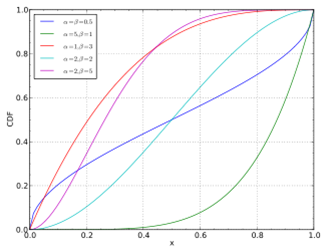
\includegraphics[scale=0.5]{Beta}\caption{베타함수의 CDF}\label{Fig:1-19}
\end{figure}\\
베타분포를 수식으로 나타내면 다음과 같다. 베타분포에서 필요한 변수는 $\alpha, \beta$가 된다.
\begin{align}
&P(\theta)=\frac{\theta^{\alpha-1}(1-\theta)^{\beta-1}}{B(\alpha ,\beta)}\label{eq:1-17}\\
&B(\alpha ,\beta)=\frac{\Gamma(\alpha)\Gamma(\beta)}{\Gamma(\alpha+\beta)}\label{eq:1-18}\\
&\Gamma(\alpha)=(\alpha -1)!\label{eq:1-19}
\end{align}
이 수식에서 $\Gamma(\alpha)$는 정수의 팩토리얼로 구할 수 있고 이를 통해 $B(\alpha,\beta)$를 구할 수 있고 이를 통해 $P(\theta)$도 구할 수 있다.
이제 수식 \eqref{eq:1-2}와 수식 \eqref{eq:1-17}을 곱하여 수식 \eqref{eq:1-16}을 구해보면 다음 결과가 나온다.
\begin{align}
P(\theta| D)\propto P(D| \theta)P(\theta)&\propto \theta^{a_H}(1-\theta)^{a_T}\theta^{\alpha-1}(1-\theta)^{\beta-1}\label{eq:1-20}\\
&=\theta^{a_H+\alpha-1}(1-\theta)^{a_T+\beta-1}\label{eq:1-21}
\end{align}
그리고 바로 위의 식을 통해 흥미로운 사실을 확인할 수 있다. 바로 $P(D| \theta)$의 값과 $P(\theta| D)$의 결과가 유사한 형태로 $\theta$와 $(1-\theta)$의 자승만 다르게 나온다는 것이다.\\

% 슬라이드 25
\noindent 그러자 이 과정을 지켜보던 억만장자가 말했다.
\begin{itemize}
\item``잠시만요. 지금 수식에 대해서 얘기하고 있는데, 나는 가장 가능성이 있고 정확한 $\theta$를 원하는 겁니다.''
\end{itemize}
그렇다면 당신은 이렇게 얘기할 수 있다.
\begin{itemize}
\item``우리는 지금 그 일을 하고 있습니다. 앞서 MLE에서는 우리는 $\theta$를 수식 \eqref{eq:1-5}을 통해서 구해서 수식 \eqref{eq:1-11}를 구해냈습니다. 그리고 지금은 MAP 관점에서 $\theta$를 수식 $\hat{\theta}=argmax_{\theta}P(\theta| D)$를 통해 구하는 것입니다. 그리고 $P(\theta| D)$는 수식 \eqref{eq:1-20}을 통해 다음과 같이 구할 수 있습니다.''
\end{itemize}
\begin{align}
P(\theta| D)\propto \theta^{a_H+\alpha-1}(1-\theta)^{a_T+\beta-1}\\
\hat{\theta}=\frac{a_H+\alpha-1}{a_H+\alpha+a_T+\beta-2}
\end{align}
\indent 여기서 $\hat{\theta}$를 구하는 과정을 좀 더 설명하면 수식 $\theta^{a_H+\alpha-1}(1-\theta)^{a_T+\beta-1}$은 수식 $\theta^{a_H}(1-\theta)^{a_T}$에서 자승 값만 바뀐 형태이므로 $\hat{\theta}$는 마찬가지로 수식 \eqref{eq:1-11}에서\\ ${a_H}\rightarrow{a_H+\alpha-1}, {a_T}\rightarrow{a_T+\beta-1}$로 바꿔주기만 하면 된다.

% 슬라이드 26
\begin{figure}[ht]\centering
\parbox[t]{4cm}{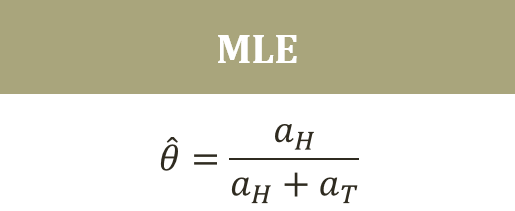
\includegraphics[scale=0.50]{MLE}\caption{MLE로 구한 $\hat{\theta}$}\label{Fig:1-20}}\hspace{1cm}
\parbox[t]{4cm}{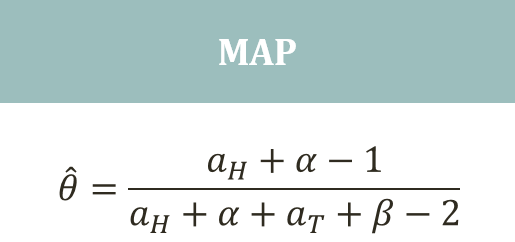
\includegraphics[scale=0.44]{MAP}\caption{MAP로 구한 $\hat{\theta}$}\label{Fig:1-21}}\\
\end{figure}
\noindent 지켜보던 억만장자가 말했다.
\begin{itemize}
\item``잠깐만요, 그렇다면 뭐가 맞는 거죠? MLE로 구한 값과 MAP로 구한 값이 다른데요?''
\end{itemize}
Bayes는 말했다.
\begin{itemize}
\item``사실 그렇진 않습니다. 이 게임을 똑같이 복제해서 많이 돌릴 수만 있다면 차이가 없습니다.''
\end{itemize}
당신도 이렇게 말할 수 있다.
\begin{itemize}
\item``그렇습니다. 만약 $a_H$와 $a_T$가 커진다면 $\alpha$와 $\beta$는 상대적으로 매우 작아져 아무것도 아니게 됩니다."
\end{itemize}
이 말을 들은 억만장자가 말했다.
\begin{itemize}
\item``만약 제가 더 많은 시도를 하지 않는다면, $\alpha$와 $\beta$가 중요하다는 말이군요. 그럼 $\alpha$와 $\beta$는 누가 결정하는 거죠?''\\
\end{itemize}

\indent 안타깝게도 $\alpha$와 $\beta$는 압정 게임의 관계자가 아닌 이상 우리는 알지 못할 것이다. 하지만 사전 정보를 주는 것은 아주 중요한 과정이다. 그럼에도 불구하고 우리는 많은 경우에 크게 신경을 쓰지 않고 있기도 하다. 그렇지만 중요한 것은 MLE와 MAP의 결과가 다르게 나올 수 있다는 것이다. 또한 MAP의 경우는 사전 지식이 들어가다보니 유용할 수도 있지만 잘못된 사전 지식을 택한다면 좋지 않은 결과물을 만들어 낼 수도 있다.\\

\subsection{확률 분포}
% 슬라이드 28
\indent 앞서 우리는 억만장자와 Bayes와 함께 압정 문제에 대해서 이야기를 나눴다.  억만장자는 작은 데이터셋을 분석하여 높은 확률로 돈을 벌고자 했고, 우리는 억만장자에게 가장 가능성 있고 정확한 답을 주려고 하였다. 그리고 Bayes는 답에 사전 지식이 포함되어야 한다는 것을 우리에게 설득을 하였다. 
\indent 결국 압정 게임의 본질을 찾고자 하였고, 중요한 키포인트는 압정을 던진 결과가 Head인지 Tail인지에 대한 확률이었다. 결국 이 문제는 확률과 관련된 문제이므로, 이 문제를 해결하기 위한 중요한 지식들은 확률과 분포 그리고 그 외 수학적인 요소들이 있다. 이를 위해서 우리는 확률과 관련된 기본적인 지식들을 다루고자 한다.\\

% 슬라이드 29
\subsubsection{확률}
\indent 먼저 가장 중요한 개념인 확률에 대한 정의부터 확립해보고자 한다. 확률은 철학적인 관점과 수학적인 관점으로 볼 수 있다. 철학적으로 보면 두가지 관점을 볼 수 잇다. 한 관점은 사건의 상태를 설명하기 위해 객관주의자가 숫자를 할당하는 것으로 Counting이라고도 한다. 다른 관점은 주관주의자가 자신만의 신념으로 숫자를 할당하는 것으로 Betting이라고도 한다.\\
\begin{figure}[ht]\centering
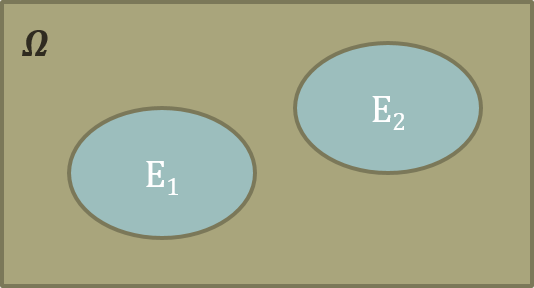
\includegraphics[scale=0.50]{Probability}\caption{사건과 확률}\label{Fig:1-22}
\end{figure}\\
\indent 한편 수학적으로 보면 확률은 아래 특성을 가진 함수가 된다.
\begin{align}
&P(E)\in R\label{eq:1-24}\\
&P(E)\geq 0\label{eq:1-25}\\
&P(\Omega)=1\label{eq:1-26}\\
P({E_1}\cup{E_2}\cup&\cdots)=\sum_{i=1}^{\infty} P(E_i)\label{eq:1-27}
\end{align}
\indent 여기서 $P$는 함수의 역할을 하게 된다. 각 수식에 대해서 간단한 설명을 덧붙이자면, 수식 \eqref{eq:1-24}와 \eqref{eq:1-25}는 어떤 사건 E가 일어날 확률은 실수이고 0보다 크다는 것이다. $\Omega$는 일어날 수 있는 모든 사건들을 합한 것으로, 수식 \eqref{eq:1-26}은 모든 사건들을 합한 것에 대한 확률은 1이라는 것이다. 그리고 수식 \eqref{eq:1-27}은 서로 상호 배반(Mutually exclusive)적인 사건들 $E_i$에 대해서 각 사건들의 합집합의 확률은 각각의 확률을 더한것과 같다는 것이다. 다음으로 확률과 관련된 몇가지 특성을 알아보도록 하겠다.
\begin{align}
if\ A\subseteq B,\ &then\ P(A)\leq P(B)\label{eq:1-28}\\
&P(\emptyset)=0\label{eq:1-29}\\
0&\leq P(E)\leq1\label{eq:1-30}\\
P(A\cup B)=P(A&)+P(B)-P(A\cap B)\label{eq:1-31}\\
P(E^C&)=1-P(E)\label{eq:1-32}
\end{align}
\indent 각 특성에 대해 간단하게 설명해보자면, 수식 \eqref{eq:1-28}은 $A$라는 사건이 $B$라는 사건에 포함될 때, $A$가 일어날 확률은 $B$가 일어날 확률보다 작다는 것이다. 쉽게 예시를 들어보면 $B$라는 사건이 자녀를 낳는 사건이고, $A$라는 사건이 딸을 낳는 사건이라고 생각하면, $A$는 $B$에 포함되고 $P(A)$는 $P(B)$보다 작게 된다. 수식 \eqref{eq:1-29}에서 $\emptyset$은 Null Event(공사건)으로 절대로 나올 수 없는 사건을 의미한다. 따라서 이에 대한 확률은 0이 되어야 한다. 그리고 수식 \eqref{eq:1-30}이 의미하는 바는 모든 사건들은 일어날 확률이 0과 1사이라는 것이다. 수식 \eqref{eq:1-31}은 집합에서 두 집합의 합집합에 대한 관계가 확률 함수를 적용해서도 유지되는 것을 보여준다. 마지막으로 수식 \eqref{eq:1-32}은 특정 사건 $E$이 있을 때 $E$가 아닌 다른 모든 사건들을 모은 것이 $E^C$가 되고 이 확률은 전체 확률 1에서 $E$의 확률을 뺀 것이 된다.\\

% 슬라이드 30
\subsubsection{조건부 확률}
\begin{figure}[ht]\centering
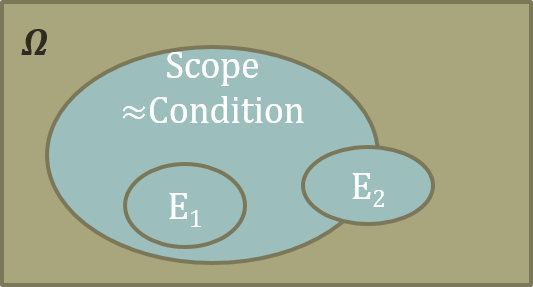
\includegraphics[scale=0.50]{Conditional_Probablilty}\caption{조건부 확률}\label{Fig:1-23}
\end{figure}
\indent 이제 조건부 확률에 대해 알아보도록 하겠다. 우리는 보통 모든 사건을 모아둔 $\Omega$를 다루지 않는다. 많은 경우 우리는 조건을 고려하며 확률을 계산을 한다. 
그림 18 에서 보면 커다란 원은 우리가 제한한 조건(Condition)을 의미한다. 만약 이 조건 안에서의 확률을 알고자 한다면, $E_1$의 경우는 전체 확률이 모두 반영이 되겠지만, $E_2$의 경우는 전체 중 조건에 포함되는 일부분 만이 확률로 계산이 될 것이다. 이를 수식으로 좀 더 명확히 확인해보도록 하겠다.
\begin{equation}
P(A|B)=\frac{P(A\cap B)}{P(B)}
\end{equation}
\indent 위 수식의 의미를 살펴보면 좌변의 $P(A|B)$는 $B$라는 조건이 참인 내부에서 $A$가 발생할 확률을 의미한다. 이 값은 결국 $B$의 영역에서 $A$와 $B$의 교집합이 발생할 확률을 의미하므로 우변의 식이 유도가 되는 것이다. 그림 22에서 참고하자면 Condition=$B$, $E_2=A$라고 볼 수 있다. 이제 조건부 확률과 관련된 몇가지 유용한 공식에 대해서 다뤄보도록 하겠다.
\begin{align}
P(B|A)=\frac{P(A|B)P(B)}{P(A)}\label{eq:1-34}\\
P(A)=\sum_{n} P(A|B_n)P(B_n)\label{eq:1-35}
\end{align}
\indent 위 공식들은 앞으로 많이 다룰 공식들이다. 수식 \eqref{eq:1-34}의 유도는 그렇게 어렵지 않으므로 한 번 시도해 보는 것을 추천한다. 수식 \eqref{eq:1-35}의 유도 역시 비슷한 방법으로 해결 가능하므로 책에서 다루진 않겠다. 수식 \eqref{eq:1-34}를 보면 조건 사건과 타겟 사건이 바뀔 수 있다는 것을 확인할 수 있다. 그리고 수식 \eqref{eq:1-35}를 보면 타겟 사건이 여러 조건과 조건부 확률의 곱들을 더함으로써 표현이 가능하다는 것을 확인할 수 있다. \\

% 슬라이드 31
\subsubsection{확률분포}
\indent 지금까지는 $P$라는 함수의 여러가지 특성에 대해서 알아보았다. 이제는 $P$라는 함수 자체의 mapping(사상)에 대해 정의를 해보도록 하겠다. 이를 Probability Distribution(확률분포)라고 한다. 확률분포는 임의적 시행이나 실험, 설문조사 등으로 나온 사건들의 집합에 대한 확률을 배정한다. 이 함수는 정의역의 사건을 공역의 확률로 mapping(사상)하는 역할을 한다. 사건이라 함은 설문조사나 실험, 시행등에서 얻어지는 연속적인 숫자 값도 될 수 있고 불연속적인 카테고리 값이 될 수도 있다. \\
\indent 예를 들어 다음 $f(x)$ 함수를 보면, $f$가 probability distribution function(확률분포함수)가 되고 $x$가 사건의 한 종류로서 이 경우에는 연속적인 값이 된다. 그리고 $f(x)$는 사건 x에 해당하는 확률 값이 된다.\\
\begin{equation}
f(x)=\frac{e^{-\frac{1}{2} x^2}}{\sqrt{2\pi}}
\end{equation}
\indent 이 함수 $f(x)$에 해당하는 확률밀도함수(PDF)와 누적분포함수(CDF)는 다음 그림과 같다. 확률밀도함수는 각 사건(x)에 대해 확률 값을 가질 수 있다. 그리고 누적분포함수는 해당 값(x)까지의 확률값을 누적하여 더한 값이다. 즉, x보다 작거나 같은 확률을 의미한다.
\begin{figure}[ht]\centering
\parbox[t]{4cm}{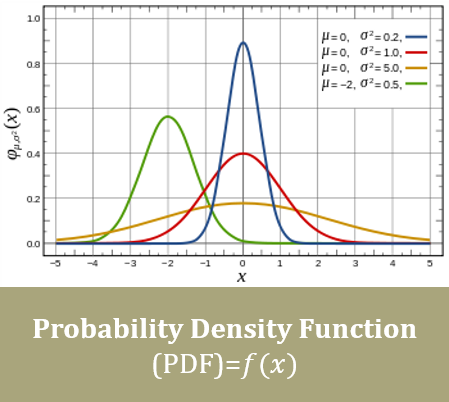
\includegraphics[scale=0.6]{PDF}\caption{확률밀도함수}\label{Fig:1-24}}\hspace{1cm}
\parbox[t]{4cm}{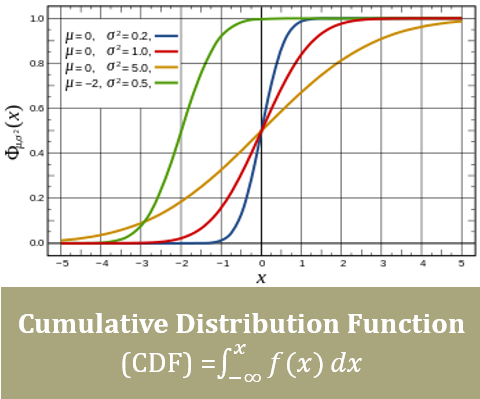
\includegraphics[scale=0.6]{CDF}\caption{누적분포함수}\label{Fig:1-25}}
\end{figure}\\

% 슬라이드 32
\indent 이와 같이 PDF와 CDF를 정할 수 있는데, 이는 매우 다양하게 정의할 수 있다. 이렇게 다양한 함수를 만들어 내는 방법에는 크게 2가지 방법이 있다. 첫번째로는 함수의 공식을 정해놓고 parameter(매개변수)를 바꾸는 방법이 있다. 두번째로는 함수의 공식 자체를 바꾸는 방법이 있다. 그리고 특정 PDF를 가지는 공식들에 대해서 이름이 붙어있는 경우도 있다. 예를 들어 Normal Distribution(정규 분포), Poisson Distribution(포아송 분포) 등이 있다. 이제 앞으로 몇가지 확률 분포들에 대해서 알아보도록 하겠다.\\
\subsubsection{정규분포}
\begin{figure}[ht]\centering
\parbox[t]{5.2cm}{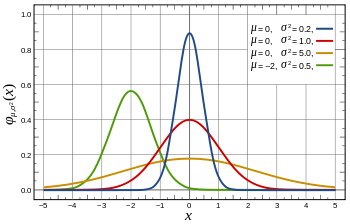
\includegraphics[scale=0.55]{Normal_PDF}\caption{정규분포의 확률밀도함수}\label{Fig:1-26}}\hspace{0.5cm}
\parbox[t]{5.2cm}{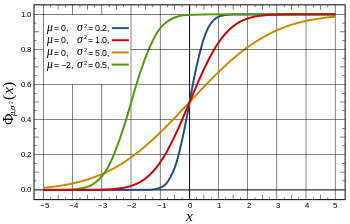
\includegraphics[scale=0.55]{Normal_CDF}\caption{정규분포의 누적분포함수}\label{Fig:1-27}}
\end{figure}
\indent 먼저 우리가 가장 많이 사용하는 정규분포에 대해서 알아보겠다. 정규분포의 식은 다음과 같다. 여기서 $mu$와 $sigma$가 parameter(매개변수)로 작용하고 Notation은 정규분포를 표시하는 방법이다. Mean과 Variance는 각각 평균과 분산을 의미한다.
\begin{align}
&f(x;\mu,\sigma)=\frac{1}{\sigma\sqrt{2\pi}} e^{-\frac{{x-\mu}^2}{2\sigma^2}}\label{eq:1-37}\\
&Notation : N(\mu,\sigma^2)\\
&Mean : \mu\\
&Variance : \sigma^2
\end{align}
\\

% 슬라이드 33
\subsubsection{베타분포}
\begin{figure}[ht]\centering
\parbox[t]{5.2cm}{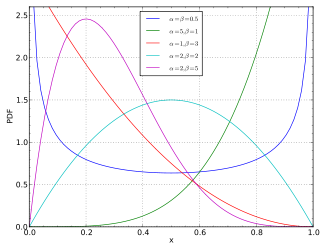
\includegraphics[scale=0.55]{Beta_PDF}\caption{베타분포의 확률밀도함수}\label{Fig:1-28}}\hspace{0.5cm}
\parbox[t]{5.2cm}{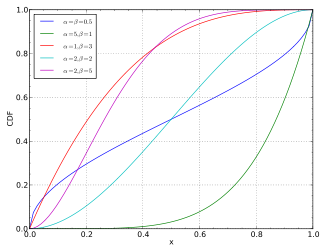
\includegraphics[scale=0.55]{Beta_CDF}\caption{베타분포의 누적분포함수}\label{Fig:1-29}}
\end{figure}
\indent 다음으로 베타분포가 있다. 베타분포와 정규분포는 비슷한 점도 있지만 다른 점이 있다. 정규분포는 정의역의 범위가 무한대인데 베타분포는 정의역의 범위가 [0,1]로 정해져있다. 이는 확률을 모델링 할 때 매우 좋은 특징으로 볼 수 있다. 그 이유는 확률은 0에서 1의 값을 가지게 되는데 베타분포의 정의역이 이와 맞는 [0,1]이기 때문이다. 베타분포의 공식들은 다음과 같다. 여기에서는 $\alpha$와 $\beta$가 매개변수로 작용한다.\\
\begin{align}
&f(\theta ;\alpha,\beta)=\frac{\theta^{\alpha -1}(1-\theta)^{\beta -1}}{B(\alpha,\beta)}\label{eq:1-38}\\
&B(\alpha,\beta)=\frac{\Gamma(\alpha)\Gamma(\beta)}{\Gamma(\alpha +\beta)}\label{eq:1-39}\\
&\Gamma(\alpha)=(\alpha -1)!\label{eq:1-40}\\
&Notation:Beta(\alpha,\beta)\label{eq:1-41}\\
&Mean:\frac{\alpha}{\alpha+\beta}\label{eq:1-42}\\
&Variance:\frac{\alpha\beta}{(\alpha+\beta)^2(\alpha+\beta+1)}\label{eq:1-43}
\end{align}
\\

% 슬라이드 34
\subsubsection{이항분포}
\begin{figure}[ht]\centering
\parbox[t]{5.2cm}{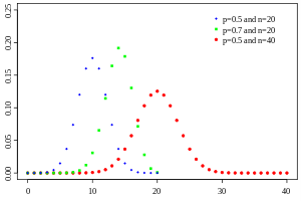
\includegraphics[scale=0.55]{Binomial_PDF}\caption{이항분포의 확률밀도함수}\label{Fig:1-30}}\hspace{0.5cm}
\parbox[t]{5.2cm}{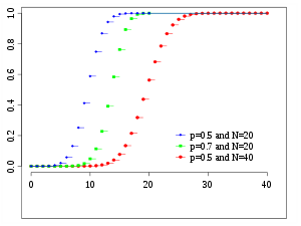
\includegraphics[scale=0.55]{Binomial_CDF}\caption{이항분포의 누적분포함수}\label{Fig:1-31}}
\end{figure}
\indent 그 다음으로 이항분포가 있다. 이항분포는 불연속적인 값을 나타내는 가장 간단한 분포이다. 따라서 위의 그림 28, 29를 보면 분포가 곡선 형태가 아닌 점 형태로 찍혀 있음을 확인 할 수 있다. 그리고 이항분포의 각 시행은 베르누이 시행이라고 불리우며 [yes or no]나 [0 or 1]과 같이 두 가지 결과만이 나와야 한다. 이항분포는 앞서 압정 문제를 풀 때 많이 다뤘던 분포이기도 하다. 이항분포의 공식들은 다음과 같다. 여기서 $n$과 $p$가 매개변수로 작용한다.
\begin{align}
&f(\theta;n,p)={\binom{n}{k}}p^k(1-p)^{n-k},\\
{\binom{n}{k}}=\frac{n!}{k!(n-k)!}\label{eq:1-44}\\
&Notation:B(n,p)\label{eq:1-45}\\
&Mean:(np)\label{eq:1-46}\\
&Variance:np(1-p)\label{eq:1-47}
\end{align}

% 슬라이드 35
\subsubsection{다항분포}
\indent 마지막으로 다항분포가 있다. 다항분포는 이항분포와 달리 2가지 선택지보다 많은 선택지가 있는 경우이다. 즉, 이항분포를 좀 더 일반화 시킨 경우이다. 예를 들면 A부터 Z까지 선택지가 있을 때 한 선택지를 고르는 경우나 여러개의 군집이 있을 때 한 군집을 선택하는 경우 등이 다항분포의 예시이다. 다항분포의 공식들은 다음과 같다. 여기에서는 $n$과 $p_i$가 매개변수로 작용한다.
\begin{align}
&f(x_1,\ldots,x_k;n,p_1,\ldots,p_k)=\frac{n!}{x_1!\ldots_k!} {p_1}^{x_1}\ldots{p_k}^{x_k}\label{eq:1-48}\\
&Notation:Mult(P),P=<p_1,\ldots,p_k>\label{eq:1-49}\\
&Mean:E(x_i)=np_i\label{eq:1-50}\\
&Variance:Var(x_i)=np_i(1-p_i)\label{eq:1-51}
\end{align}

% 슬라이드 36
\section*{Acknowledgement}
\noindent This material is greatly influenced by
\begin{itemize}\setlength\itemsep{-\parsep}
\item Professor Carlos Guestrin at CMU \\
\item Professor Eric P. Xing at CMU
\end{itemize}
\indent Some images are copied from the lecture slides made by
\begin{itemize}\setlength\itemsep{-\parsep}
\item Professor Carlos Guestrin at CMU \\
\item Professor Eric P. Xing at CMU
\end{itemize}

% 슬라이드 37
\section*{Further Readings}
\begin{itemize}
\setlength\itemsep{-\parsep}
\item Bishop Chapter 1,2
\end{itemize}
\end{document}
